\section{Experiments}
\label{sec:experiments}

\subsection{Data}

We're using the *BigEarthNet dataset* % source BigEarthNet
for our evaluations. The goal is to use the model as a feature generator and use these features for solving the multi-label classification problem with 19 classes from BigEarthNet. This dataset contains around 550.000 image patches from Sentinel-I and Sentinel-II with multi-class labels for every image. We are going to use the *Sentinel-I* images for our experiments.


The data is split into train and test set based on the implementation from the torchgeo repository. %https://torchgeo.readthedocs.io/en/latest/api/datasets.html#bigearthnet
The train dataset contains around 270.000 and the test dataset has 125.000 images.

There are high differences in the occurrence of certain classes in the dataset (see \ref{fig:class-distribution}). There are, for example, only a few images with wetlands, beaches, and moors. The metrics during the evaluation have to account for this.

\begin{figure}
  \centering
  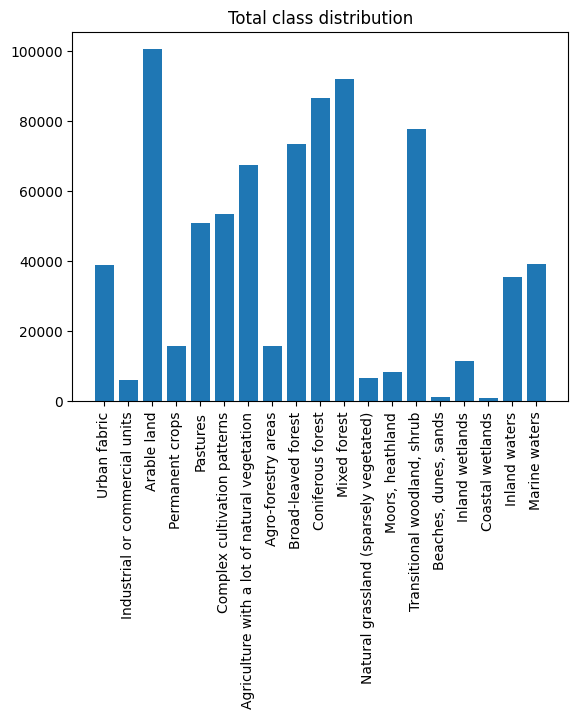
\includegraphics[width=\linewidth]{images/class_distribution.png}
  \caption{Distribution of the classes in the train dataset. This is a multiclass dataset so one can have multiple classes.}
  \label{fig:class-distribution}
\end{figure}

\begin{figure}
  \centering
  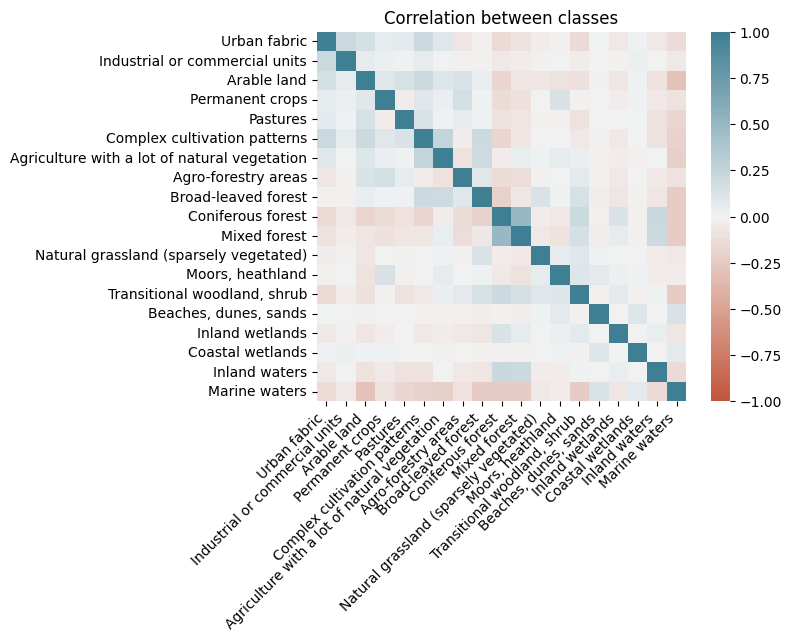
\includegraphics[width=\linewidth]{images/correlation.png}
  \caption{Correlation of classes in the train dataset}
  \label{fig:correlation}
\end{figure}

We analyzed the correlation between classes of BigEarthNet and the results are displayed in \ref{fig:correlation}. The classes are mostly uncorrelated with some exceptions like the high likeliness that coniferous forests are usually also mixed forests and marine waters are mostly not in the same images as all the other vegetation forms.

\subsection{Performance Metrics}

We decided to compute multiple metrics for evaluating the performance of the models in the classification tasks. We provide results for *f2-micro, f2-macro* (see XXXX for implementation) % https://scikit-learn.org/stable/modules/generated/sklearn.metrics.fbeta_score.html
*, hamming-loss*, and *precision * scores (see XXXX for implementation) % https://scikit-learn.org/stable/modules/generated/sklearn.metrics.precision_score.html
. We also calculate precision and f1 scores for individual classes.

\subsection{Results}

First, we calculated feature vectors using DOFA for all the images in BigEarthNet (Sentinel-I) and saved them for further use. All the following analyses use these vectors for visualizations or the downstream classification task.

\subsubsection{UMAP Feature analysis}

\begin{figure}
  \centering
  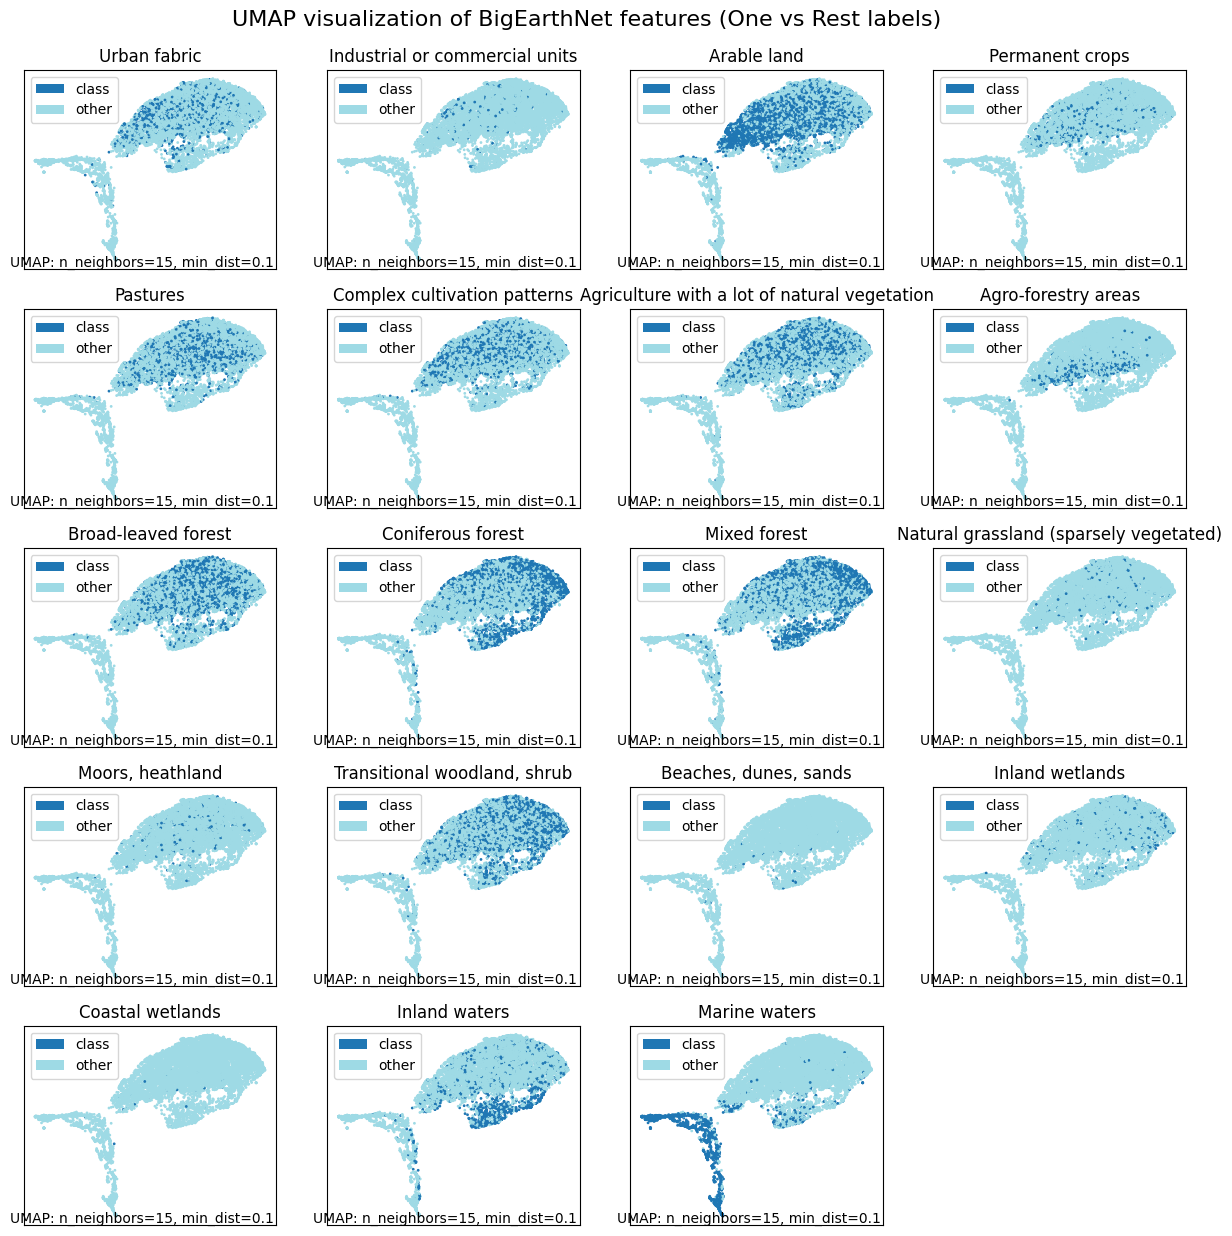
\includegraphics[width=\linewidth]{images/umap.png}
  \caption{Visualization of the 19 classes in a UMAP transformed space (one vs. rest)}
  \label{fig:umap}
\end{figure}

In \ref{fig:umap} are the occurrences of different classes in a UMAP transformed 2D space visualized. Because one image has multiple labels we choose the visualization via multiple charts. In this visualization, we expect different classes to be in different data cloud regions. As we can see this holds for a lot of the classes. Most notably we have a separate region for all marine water images (right bottom chart). As we've seen in @correlation this class is negatively correlated with most of the other classes so a separation in this visualization is plausible.
It appears that arable land is more on the left side of the main region while forests, woodlands, etc. are more on the right side.

With the results of this visualization, we expect that the feature vectors of DOFA capture the semantic meaning of the different images and it should be possible to train a classifier on top of that data.

\subsubsection{Classification}

We used the feature vectors of DOFA to train different ML algorithms for the given classification task. All the approaches use the same data split. In @test-results are the final results of these experiments.

\begin{figure}
  \centering
  \begin{tabular}{||c c c c c||} 
    \hline
    sdsd & $F^2_{macro}$ \% & $F^2_{micro}$ \% & hamming loss & $P_{macro}$ \%  & $P_{micro}$ \% \\ [0.5ex] 
    \hline\hline
    Test & 1 & 6 & 87837 & 787 & 787 \\ 
    \hline
    Test & 2 & 7 & 78 & 5415 & 787 \\
    \hline
    Test & 3 & 545 & 778 & 7507 & 787 \\
    \hline
    Test & 4 & 545 & 18744 & 7560 & 787 \\
    \hline
    Test & 5 & 88 & 788 & 6344 & 787 \\ [1ex] 
    \hline
  \end{tabular}
  \caption{Test results of different classification approaches on the 19-class multi-label classification task \footnote{Some classes contain so few examples that they are not in the test dataset and receive a $F^2$ score of 0.}}
  \label{fig:test-results}
\end{figure}

#figure(
  table(
    columns: (auto, auto, auto, auto, auto, auto),
    inset: 3pt,
    align: horizon,
    table.header(
      [], [$F^2_"macro"$ (%)], [$F^2_"micro"$ (%)], [*hamming loss*], [$P_"macro"$ (%)], [$P_"micro"$ (%)], 
    ),
    "Random Forest",
    $21.4$,
    $35.8$,
    $0.123$,
    $52$,
    $bold(72)$,
    "Linear Probing",
    $22.9$,
    $35.3$,
    $0.124$,
    $49$,
    $70$,
    "MLP",
    $bold(34.5)$,
    $bold(47.8)$,
    $bold(0.113)$,
    $bold(58)$,
    $71$,
  ),
  caption: "Test results of different classification approaches on the 19-class multi-label classification task" + footnote("Some classes contain so few examples that they are not in the test dataset and receive a " + $F^2$ + " score of 0.")
) <test-results>

#figure(
  table(
    columns: (auto, auto, auto, auto, auto, auto),
    inset: 3pt,
    align: horizon,
    table.header(
      [], [$F^2_"macro"$ (%)], [$F^2_"micro"$ (%)], [*hamming loss*], [$P_"macro"$ (%)], [$P_"micro"$ (%)], 
    ),
    "Random Forest",
    $9.46$,
    $33.7$,
    $0.056$,
    $24$,
    $71$,
    "Linear Probing", // todo the rest of the lines
    $22.9$,
    $35.3$,
    $0.124$,
    $49$,
    $70$,
    "MLP",
    $bold(34.5)$,
    $bold(47.8)$,
    $bold(0.113)$,
    $bold(58)$,
    $71$,
  ),
  caption: "Test results of different classification approaches on the 43-class multi-label classification task"
) <test-results-43>

There are notable differences in the performance of the chosen approaches. MLP has the best performance over most of the metrics. However random forest classifier and linear probing also have similar scores in $P_"micro"$ and $P_"macro"$. All classifiers have significant differences between their micro and macro averaged scores. When we compare the $F^2$ scores per class we can see the cause for these values (@scores-by-class). There is a high variance in the performance across classes which reaches from $0%$ $F^2$ score to about $90%$ $F^2$ score. This leads to the different averaging variants resulting in different scores. We can also see that MLP manages to achieve higher scores than the linear classifier over more classes.

#figure(
  grid(
    columns: (auto, auto),
    rows: (auto),
    gutter: 3pt,
    image("images/Linear Probing - f2 scores.png"),
    image("images/MLP - f2 scores.png"),
  ),
  caption: $F^2$ + " scores for every class. Left side for the linear classifier, right side for the MLP classifier."
) <scores-by-class>

This leads to the conclusion that the features generated by the DOFA model are not well linearly separable across all classes and only some achieve a $F^2$ score of over $50%$.

Random forest classifiers can separate high dimensional data, but in this case, their scores are on the same level as the linear classifier. // WHY????

#figure(
  image("images/MLP - confusion matrix.png"),
  caption: "Confusion matrices of the MLP classifier on the test set. The matrices are calculated separately for each class."
)

// REMARKS ABOUT CONFUSION MATRIX